\chapter{Numerical Methods}

\section{Introduction}

This chapter focuses on the methods that are used for the numerical computations in this thesis.
In order to compute the temporal evolvement of a fluid system from its initial state, it is necessary to discretize
the equations of motion by using different numerical schemes.\\
For this purpose various discretization approaches, for example finite-element and finite-volume methods, exists.
Here we will introduce the method of finite-difference stencils for the spatial and a third order Runge-Kutta method for the discretization in time.
Furthermore we will introduce the method of artificial compressibility, which can be used to avoid the numerical expensive solution of a poisson equation.
The choice of these methods in combination with the usage of cartesian grids is in particular time saving when performing computations on the gpu, as we
will see in chapter \ref{chapter:cuda}.

\section{Finite Differencing Schemes}

We start with a brief introduction of finite difference methods.
The interested reader is referred to \citep{ferziger99} for a more general overview, from where this section is adapted.
The partial differential equations we want to solve in this thesis are of the form,

\begin{align}
    \label{numerik:pde_allg}
    \pdn[\Phi]{t} = \left(\sum_{x_i=x,y,z}\left( A_i \pdn[]{x_i}  + B_i \pdn[^2]{x_i^2}\right) + C +  \vec{u}\vec{\nabla} \right) \Phi = \mathcal{L} \Phi
\end{align}
    %\pdn[\Phi]{t} = A \pdn[^2\Phi]{x^2}  + B \pdn[^2\Phi]{x^2}     + C(\vec{r}, \vec{u}, t) +  \vec{u}\left(\pdn[^2\Phi]{x^2} +  \pdn[^2\Phi]{x^2} + \pdn[\Phi]{x}\right) = \mathcal{L}

where $\Phi(\vec{r}, t)\in\mathbb{R}$ and $\mathcal{L}$ is a differential operator, containing spatial derivatives up to second order.
The numerical integration can be divided into two steps, the calculation of $\mathcal{L}$, which we want to discuss in this
section and secondly the integration in time.
The exact calculation of the spatial derivatives in $\mathcal{L}$ is numerically not possible.\\
Due to the limited storage capacity and computation time of computers,
it is necessary to discretize the domain, on which the PDE should be solved and find a adequate approximation of these operators.
Here we will fall back to the  one-dimensional case, the implementation for three dimensions will be discussed in chapter \ref{chapter:cuda}.\\

Let $\Omega = \{x \in \mathbb{R} \;|\; 0 \leq x \leq L\}$ be the domain on which we want to solve equations of the type \ref{numerik:pde_allg}.
For the discretization we divide $\Omega$ into $N$ equidistant points $x_i = \sum_i \Delta x_i$, with the position index ${i\in\{[0, N-1]|i\in\mathbb{N}\}}$
and $\Delta x_i = x_{i+1} - x_i = L/(N-1)$.
\footnote{EVTL?}
We assume that $\Phi$ is a  continuous differentiable function.
Local to a grid point $x_i$ and $\Phi$ can than be expressed with a Taylor series [CITE].

\begin{align}
    \label{num:taylor}
    \Phi(x) = \sum_{n=0}^{\infty} \pdn[^n\Phi(x_i)]{x^n} \frac{(x - x_i)^n}{n!}
\end{align}

By evaluating the Taylor expansion at different points, we obtain expressions for the first derivative. For example
a combined evaluation at the points $x_{i+1}$, $x_{i-1}$ leads to the expression

\begin{align}
    \label{num:cds}
    \left.\left(\pdn[\Phi]{x}\right)\right|_{i} = \frac{\Phi_{i+1} - \Phi_{i-1}}{x_{i+1} - x_{i-1}}
     - \frac{(x_{i+1} - x_i)^2 - (x_i - x_{i-1})^2}{2 (x_{i+1} - x_{i-1})}\left(\pdn[^2\Phi]{x^2}\right)_i + \mathcal{O}(\Delta x^3)
\end{align}

For a constant grid size, that is $\Delta x := \Delta x_i = \text{const.}$, the second order term in equation \ref{num:cds} vanishes.
By neglecting all terms of higher order, we obtain a approximation for $\partial_x \Phi$ of second order.
This is the so-called central-difference (CDS) scheme. A single point evaluation of \ref{num:taylor} at $x_{i+1}$ and $x_{i-1}$, results in the forward- (FDS) and
backward- (BDS) scheme of first order. A comparison of the FD-schemes is given in table \ref{num:df_table}


\bgroup\large
\begin{table}[!tbp]
\centering
\def\arraystretch{2.2}%
\begin{tabular}{c c c c c}\toprule
Scheme-Name & Stencil & Truncation Error & Evaluation at\\[0.5ex]
\midrule
Forward  (FDS) & $\left(\pdn[\Phi]{x}\right)_i =  \frac{f_{i+1} - f{i}}   {\Delta x}$ & $\mathcal{O}(\Delta x)$  &$x_{i+1}$\\
Backward (BDS) & $\left(\pdn[\Phi]{x}\right)_i = \frac{f_{i}    - f_{i-1}}{\Delta x}$  &$ \mathcal{O}(\Delta x)$ & $x_{i-1}$\\\
Central  (CDS) & $\left(\pdn[\Phi]{x}\right)_i = \frac{f_{i+1}  - f_{i-1}}{2\Delta x}$ &$ \mathcal{O}(\Delta x^3)$& $x_{i+1}$ \& $x_{i-1}$\\
\\
\bottomrule
\label{num:df_table}
\end{tabular}
\caption{Different FD-Schemes}
\end{table}
\egroup

\begin{figure}[!btp]
  \centering
    \resizebox{0.9\textwidth}{!}{
   \import{gfx/numerik/}{finite_differenzen.pdf_tex}
  }
  \caption{Approximation of the function $\Phi$ by different finite difference schemes.}
  \label{num:fd_image}
\end{figure}

The numerical error which is made by neglecting the higher order terms, is in general referred to as the truncation error of a FD-scheme.
It should be noted that the number of grid points used for the approximation, does significantly affect the resulting error.\\
Finally figure \ref{num:fd_image} shows a visual comparison for the three different stencils.
This example once again illustrates that when approximating a function, which contains higher order terms i.e. at a local maximum,
the  CDS-scheme gives better results.\\
For the computation of the second derivative, one approach is to evaluate equation \ref{num:taylor} halfway between two points at the positions $x_{i\pm\frac{1}{2}}$

\begin{align}
    \label{numerik:eq_2dfo2}
    \left.\left(\pdn[^2\Phi]{x^2}\right)\right|_{x_i} =
     \frac{\left.\left(\pdn[\Phi]{x}\right)\right|_{i+\frac{1}{2}}-
     \left.\left(\pdn[\Phi]{x}\right)\right|_{i-\frac{1}{2}}}
    {\frac{1}{2}(x_{i+1} - x_{i-1})} + \mathcal{O}(\Delta ^2)  \approx
    \frac{\Phi_{i+1} - 2\Phi_i + \Phi_{i-1}}{\Delta x^2}
\end{align}

For the approximation of the first derivatives, it is necessary to use the FDS-scheme at $x_{i+1/2}$ and the BDS-scheme at $x_{i-1/2}$ to obtain
a second order accuracy.\\
So far we introduced methods up to an accuracy of second order. The fourth order methods which are used in this thesis are given by

\begin{align}
    \left(\pdn[\Phi]{x}\right)_i &\approx \frac{-\Phi_{i+2} + 8\Phi_{i+1} - 8\Phi_{i-1} + \Phi_{i-2}}{12\Delta x} \\
    \left(\pdn[^2\Phi]{x^2}\right)_i &\approx \frac{-\Phi_{i+2} + 16\Phi_{i+1} -30\Phi_i + 16\Phi_{i-1} - \Phi_{i-2}}{12\Delta x^2}
    \label{num:fd_o4_methods}
\end{align}

The derivation of these equations can be performed in analogy to the second order schemes, but by using a five-point
stencil. The interested reader is referred to \citep{Fornberg1988}.

\newpage

\section{Runge-Kutta Method}

With the finite difference approximation $\mathcal{L^*}$ of the differential operator $\mathcal{L}$,
we are able to solve equation \ref{numerik:pde_allg} by separation of variables.

\begin{align}
    \Phi(t) = \Phi(0) + \int_{t_0}^{t} \mathcal{L^*} (t, \Phi(t)) \dif t
\end{align}

For a numerical computation, the integration interval $[t_0, t]$  is splitted into sub-intervals $[t^n, t^{n+1}]$ of length $\Delta t$ and integrated piecewiese.
In order to approximate the integration on a sub-intervall, we know want to introduce the use of Runge-Kutta methods based on \citep{Sarbach2012}
The idea behind this method is to iteratively evaluate $\mathcal{L^*}$ at $s$ different times $\tau_i=c_i \Delta t$ with $c_i \in \{\mathbb{R} | c_i<1  \}$,
that is
\begin{align}
 k_i = \mathcal{L^*} \left(\tau_i, \Phi(t_n) + \Delta t \left(a_{21} k_{s-1} + \dots + a_{s, s-1} k_{s-1} \right)\right)
\end{align}

By using a coefficient weighted average of the $k_i$, we obtain

\begin{align}
    \Phi(t^{n+1}) = \Phi(t) + \Delta t \left( \sum_{i=1}^s b_i k_i \right)
\end{align}

The accuracy of an s-stage runge-kutta method depends of the right choice of coefficients.
In this thesis we use a third-order accurate scheme.
The coefficients are given by the butcher tableau \citep{QUELLE}
\footnote{oder quelle}

\begin{align}
    \label{num:butcher}
    \def\arraystretch{1.5}%
    \begin{array}{c|c}
        \mathbf{c} & A\\
        \hline     & \mathbf{b^T} \\
    \end{array}
    \qquad &= \qquad
    \def\arraystretch{1.5}%
    \begin{array}{c|ccc}
            0 \\
                    \frac{1}{3} & \frac{1}{3} \\
            \frac{3}{4} & \frac{-3}{16} & \frac{15}{16} \\
            \hline & \frac{1}{6} & \frac{3}{10} & \frac{8}{15}
    \end{array}
\end{align}

For the implementation of this method, we have to concern, that we have to deal with a large number of variables.
In a three dimensional fluid domain the number of grid points scales with a power of three, with an increase in the resolution.
Therefore we want to introduce a low-storage scheme of method \ref{num:butcher},  first introduced by \citep{Williamson1980}.
By keeping the information from previous computation steps, the scheme can than be translated into an iterative algorithm,
where the required amount of storage can be reduced to two registers $\Phi$ and $Q$.

\begin{align}
    \begin{split}
    Q_1 = \Delta t \mathcal{L}^*\left(\Phi^n\right)\qquad &\Rightarrow \qquad \Phi^{1} = \Phi^n + \frac{1}{3}Q_1 \\
    \Rightarrow Q_2 = \Delta t \mathcal{L}^*\left(\Phi^1\right) - \frac{5}{9} Q_1 \qquad &\Rightarrow \qquad \Phi^{2} = \Phi^1 + \frac{15}{16}Q_2 \\
   \Rightarrow  Q_3 = \Delta t \mathcal{L}^*\left(\Phi^2\right) - \frac{153}{128} Q_2 \qquad &\Rightarrow \qquad \Phi^{n+1} = \Phi^2 + \frac{8}{15}Q_3 \\
    \end{split}
\end{align}


\section{Numerical Stability}

It is important to consider the stability of a numerical method. In general it is said that a method is numerical stable if the error
introduced by approximations and roundoff errors does not grow over time \citep{ferziger99}.\\

\subsection{Runge-Kutta Scheme}

Suppose we have stationary solution for equation \ref{numerik:pde_allg}.
The system should remain unaffected by a further integration, even with the introduction of small numerical errors.
In order to obtain a stability condition it is sufficient enough to perform a linear stability analysis.
The most common approach is to study the one-dimensional linearized and diagonalized test problem (\citep{BLABLA})

\begin{align}
\label{num:rk_stab}
\frac{\dif y}{\dif t} = \lambda \Phi
\end{align}

with the eigenvalue $\lambda \in \mathbb{C}$ of a linearized operator.
It can be shown that the discretization of equation \ref{num:rk_stab}, using a Runge-Kutta scheme of $s$-order,
results in  the mapping (\citep{BLABLA})

\begin{align}
    y_{i+1}  = \left(\sum_{p=1}^s \frac{(\Delta t \lambda)^p}{p!}  + 1 \right) y_i = f(\Delta t\lambda)y_i
\end{align}

\begin{figure}[!tp]
  \begin{minipage}[c]{0.6\textwidth}
      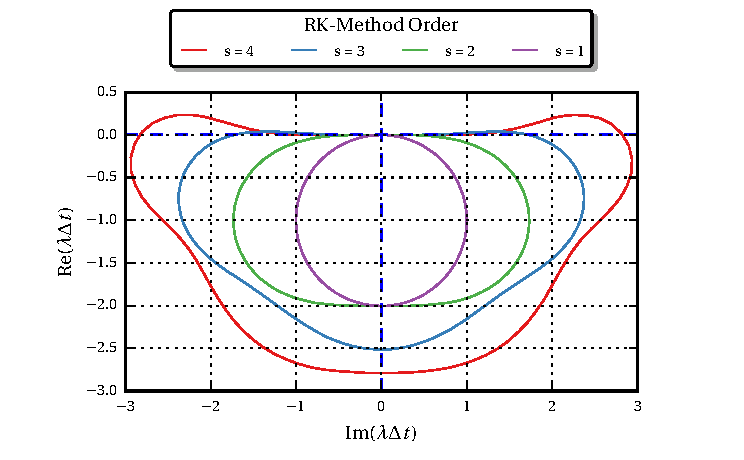
\includegraphics{gfx/numerik/rk_stability.pdf}
  \end{minipage}\hfill
  \begin{minipage}[c]{0.3\textwidth}
  \caption{Stability regions for $\Omega_s$ for different Runge-Kutta methods}
  \label{fig:num_rkstab}
  \end{minipage}
\end{figure}

The discretized system contains a stable fixed point when the condition $|f|\leq 1$ is satisfied.
Figure \ref{fig:num_rkstab} shows the different stability regions for Runge-Kutta schemes up to fourth order.
The calculation can be found in (APPENDIX)
For an $s$ order scheme the region of absolute stability is independent of the used implementation \citep{canuto2007}.
\footnote{For an $s$-th order RK-scheme different coeffiicent $a_ij$, $b_j$ and $c_i$ can be used.}
It can be noted that the stability region $\Omega_s$ increases with the uses of higher order schemes.
The substantial detail is that for method of third and fourth order, the imaginary axis lies within $\Omega_s$.
Thus these methods should be preferred for  CFD-simulations, since they tend to stabilize numerical oscillations \citep{DIPLOM}.

\subsection{Finite difference schemes}

The numerical stability of the finite difference schemes can be estimated by a Von-Neumann error analysis.
In this section the stability criterion will be exeplarily computed for a one-dimensional diffusion equation of the form
\begin{align}
    \label{num:vne_diffusion_theo}
    \pdn[v]{t} = \alpha \Delta v
\end{align}

where $\alpha$ is the diffusion coefficient. Eq.  \ref{num:vne_diffusion_theo} is discretized by
the second order central-difference scheme, given by Eq. \ref{numerik:eq_2dfo2}.
All methods and steps in this example are adopted from \citep{janderson}.
In order to test if a method is stable, it is valid to assume that the numerical error can be expressed in form of a fourier-mode.

\begin{align}
    \epsilon(x, t) = \sum_{m=1}^{N/2} \epsilon_m(x, t) \qquad &\text{and} \qquad  \epsilon_m(x, t) = e^{at}e^{i k_m x}
\end{align}

where $a$ the growth rate of the error, the wavenumber is given by $k_m=\nicefrac{2\pi m}{L}$ and $L$ is the size of the simulation domain.
The index $m$ is restricted by the domain size and the distance $\Delta x$ between two grid points, i.e. the smallest wave number
is resulting from the wavelength $\lambda=L$ and the largest from $\lambda=2\Delta x$.
Due to the linearity of the laplace operator it is sufficient to consider the stability of a single fourier mode $\epsilon_m$.
With the use of Eq.  \ref{numerik:eq_2dfo2}, the discretized version of the diffusion equations reads.
\begin{align}
    \label{num:neumann_diffusion_eq}
    \frac{\Phi^{n+1} - \Phi^n}{\Delta t} = \frac{\alpha}{\Delta x^2}\left(\Phi_{i+1}^n - 2\Phi_{i}^n + \Phi_{i-1}^n\right)
\end{align}

where $\alpha$ is the diffusion coefficient. The timestep in this example is discretized by a simple euler timestep.
Inserting $\epsilon_m$ in Eq. \ref{num:neumann_diffusion_eq} for $\Phi$ and using some trigonometric identities  gives

\begin{align}
    e^{a \Delta t} = 1 -  \frac{4\alpha \Delta t}{\Delta x^2} \sin^2\left(\frac{k_m \Delta x}{2}\right)
\end{align}

Furthermore it holds that

\begin{align}
    \left|\frac{\epsilon_i^{n+1}}{\epsilon_i^n}\right| =
    \left|\frac{e^{a(t + \Delta t)}e^{ik_mx}}{ e^{at}e^{ik_m x}}\right| = \left|e^{a\Delta t}\right|
\end{align}

The stability of the finite differenc scheme is given when the numerical error does not grow over time. This is fullfilled when the inequality

\begin{align}
    \label{num:stab_ineq}
    \left|\frac{\epsilon_i^{n+1}}{\epsilon_i^n}\right| =
    \underbrace{\left|1 -  \frac{4\alpha \Delta t}{\Delta x^2} \sin^2\left(\frac{k_m \Delta x}{2}\right)\right|}_{=:G} \leq 1
\end{align}

holds, where $G$ is denoted as the amplification factor. From the inequality from Eq. \ref{num:stab_ineq}
the stability is given by

\begin{align}
   \frac{\alpha \Delta t}{\Delta x^2} \leq \frac{1}{2}
\end{align}

From this equation it can be seen that with an increase in the resolution, the timestep has to been scaled by the square of the resolution, in order to
maintain stability. The same approach introduced for the diffusion equation can be repeated for a first-order wave equation (see \citep{janderson})
and for an advection-diffusion equation (see \citep{ferziger99}).
%Given by
%\begin{align}
%    \pdn[\Phi]{t} + c \pdn[\Phi]{x} = 0 \qquad &; \qquad  \pdn[\Phi]{t} + v \pdn[\Phi]{x}  - \frac{A}{B}\pdn[^\phi]{x^2}
%\end{align}
%where $c$ is velocitiy ect.
%By inserting the error

As a result two additional stability criterions are given.
The first one is (see \citep{janderson})
\begin{align}
   \frac{c \Delta t}{\Delta x} \leq 1
\end{align}
where $c$ denotes the maximal velocity of the system, i.e. this could be the sound speed for a compressible system.
The second criterion is given by (see \citep{ferziger99}

\begin{align}
    \Pe  < 2
\end{align}

where $ Pe := \nicefrac{u \Delta x}{\alpha}$ is defined as the Peclet number \citep{ferziger99}.
The Peclet number can be interpreted as the ratio between the advection and diffusion of a fluid system.

\paragraph{Third Order Upwinding Scheme}\mbox{}\\

For large Peclet numbers it is a common problem that numerical oscillations emerge in the numerical solution.
Additional to the central differences, the upwinding scheme, which tends to reduce
numerical oscillations, is used in this thesis. Consider the one-dimensional advection equation

\begin{align}
    \pdn[\Phi]{t} + v\pdn[\Phi]{x} = 0
\end{align}

The discretization for the advection term at the position $x=i$ is given by (see \citep{FINDQUOTE})

\begin{align}
    v\pdn[\Phi]{x} &\approx  v_i \cdot \left(\frac{2\Phi_{i+1} + 3\Phi_i     - 6\Phi_{i-1} + \Phi_{i-2}}{6\Delta x}\right)\\
\end{align}
for v(x) > 0 and
\begin{align}
    v\pdn[\Phi]{x} &\approx  v_i \cdot \left( \frac{-\Phi_{i+2} + 6\Phi_{i+1} - 3\Phi_{i-1} - 2\Phi_{i-1}}{6\Delta x}\right)
\end{align}
for v(x) < 0.

\newpage

\section{Numerical Viscosity}

In this thesis the finite difference schemes Eq.  \ref{num:fd_o4_methods} and Eq.  \ref{numerik:eq_2dfo2}
are used for the approximation of the viscous stress in the Navier-Stokes Equation.
However due to the approximation, the numerical viscosicty $D_N$ of the approximation may differ from the physical viscosity $D_P$.
An estimation for the ratio $D_N/D_P$ can be given by the following estimation. \footnote{Private communication with A.Tilgner}
Consider the  equation

\begin{align}
    \label{num:nvis_eqdiff}
    \pdn[v]{t} = D_P\pdn[^2v]{x^2}
\end{align}

A solution is given by $v = V(t)e^{ikx}$. Inserting this solution in Eq. \ref{num:nvis_eqdiff} one obtains
\begin{align}
    V(t) = V_0 \exp^{-D_Pk^2t}
\end{align}

By inserting this expression into the second order approximation Eq. () it
follows that

\begin{align}
                      D_P \Delta v  &\approx \frac{D_P}{\Delta x^2} \left(v_{x+\Delta x} - 2 v_x + v_{x - \Delta x}\right) \\
    \Leftrightarrow   -D_P k^2        &\approx \frac{D_P}{\Delta x^2} \left(\exp^{ik\Delta x} - 2 + \exp^{-ik\Delta x}\right) =   \frac{D_P}{\Delta x^2} \left(2\cos(k\Delta x) - 2\right)\\
    \Rightarrow   D_P      &\approx - \frac{D_P}{k^2 \Delta x^2} \left(2\cos(k\Delta x) - 2\right)
\end{align}

From Eq. it can be seen that the numerical viscosity is given by
\begin{align}
 \label{NUMERIC:NUMVIS}
    D_N = \frac{D}{k^2 \Delta x^2} \left(2\cos(k\Delta x) - 2\right)
\end{align}
The same approach for the fourth order scheme gives
\begin{align}
 \label{NUMERIC:NUMVIS2}
    D_N = \frac{D}{k^2 \Delta x^2} \left(32\cos(k\Delta ) - 2\cos(k\Delta x) - 30\right)
\end{align}
\clearpage



\section{Method of Artificial Compressibility}

For now the fact was ignored that the equations of motion i.e. Eq.  \ref{theorie:eqns} cannot directly be solved for the pressure.
An equation for $p$ can be obtained by taking the divergence of Eq.  \ref{theorie:eqns} and apply the continuity equation.
The resulting equation is \citep{QUOTE}

\begin{align}
    \Delta p =  -\nabla \left( \sum \vec{F}_{\text{ext.}} - (\vec{u} \vec{\nabla}) \vec{u}\right)
\end{align}

In order to determine the pressure it would be necessary to solve a poisson equation.
The numerical solution  however, can be very time consuming is  furthermore difficult to implement on a GPU \citep{TILGNER}.
Instead here the method of artificial compressibility, developed by \citep{Chorin1997}, will be introduced.
The concept of this method is to introduce the artificial equations of state


   \noindent\begin{minipage}{0.4\textwidth}
        \begin{align}
            \label{num:arti_cont}
            \pdn[\rho]{t} +  \nabla \vec{v} = 0
        \end{align}
    \end{minipage}%
    \begin{minipage}{0.2\textwidth}\centering
        \begin{align}
            \label{num:arti_pressure}
              p =\rho/\delta
        \end{align}
    \end{minipage}%
    \begin{minipage}{0.2\textwidth}\centering
        \begin{align}
                c=\frac{1}{\delta^{1/2}}
        \end{align}
    \end{minipage}\vskip1em




where $\rho$ is the artifical density, $\delta$ the artificial compressibility and $c$ the artificial speed of sound.
Eq.  \ref{num:arti_cont}  is a motified version of the continuity equation and Eq. \ref{num:arti_pressure} introduces
an artificial equation for the pressure. A substitution of Eq. \ref{num:arti_pressure} into the Navier-Stokes Eq. \ref{BLA} gives

\begin{align}
    \label{numerik:nsac}
    \pdn[u]{t} + \left(\vec{u} \vec{\nabla}\right) \vec{u} &= -c^2\nabla\rho + \Rey \Delta \vec{u}+\sum \vec{F}_{\text{ext.}}
\end{align}

The system has an artificial compressibility. The idea of this method is to use a large number for $c$ such that
the mach number
\begin{align}
    M = \frac{1}{c}\max\left(\sum_i |\vec{u_i}]^2\right)^{1/2}
\end{align}

is sma

-stiff problem
-implizit methods
-problem not suited for gpus
